\chapter{Présentation du projet}


\section{Contexte}

Dans le cadre du projet DSCATT, nous Paul Chapron (IGN) Romain Reuillon (CNRS) et Etienne Delay (CIRAD) avons animé 1 semaine d'atelier à Diohine sur le territoire de l'observatoire IRD de Niakhar(fig. \ref{fig:photoAtelier}). Ils s'inscrivent dans différentes réflexions de recherche autour de l'exploration d'accompagnement, et les théories de la viabilité appliquées aux systèmes multi-agents.
Ces journées d'atelier ont mobilisé quatre acteurs locaux sur cinq jours:
\begin{itemize}
  \item Paul Sene +221 77 623 60 93
  \item Marcel Latyr Diouf +221 77 198 41 06
  \item Marie Hélène Ndjira +221 77 072 57 60
  \item Idrissa Faye +221 77 408 24 76
  \item Robert Diate
\end{itemize}


\begin{figure}
  \begin{center}
    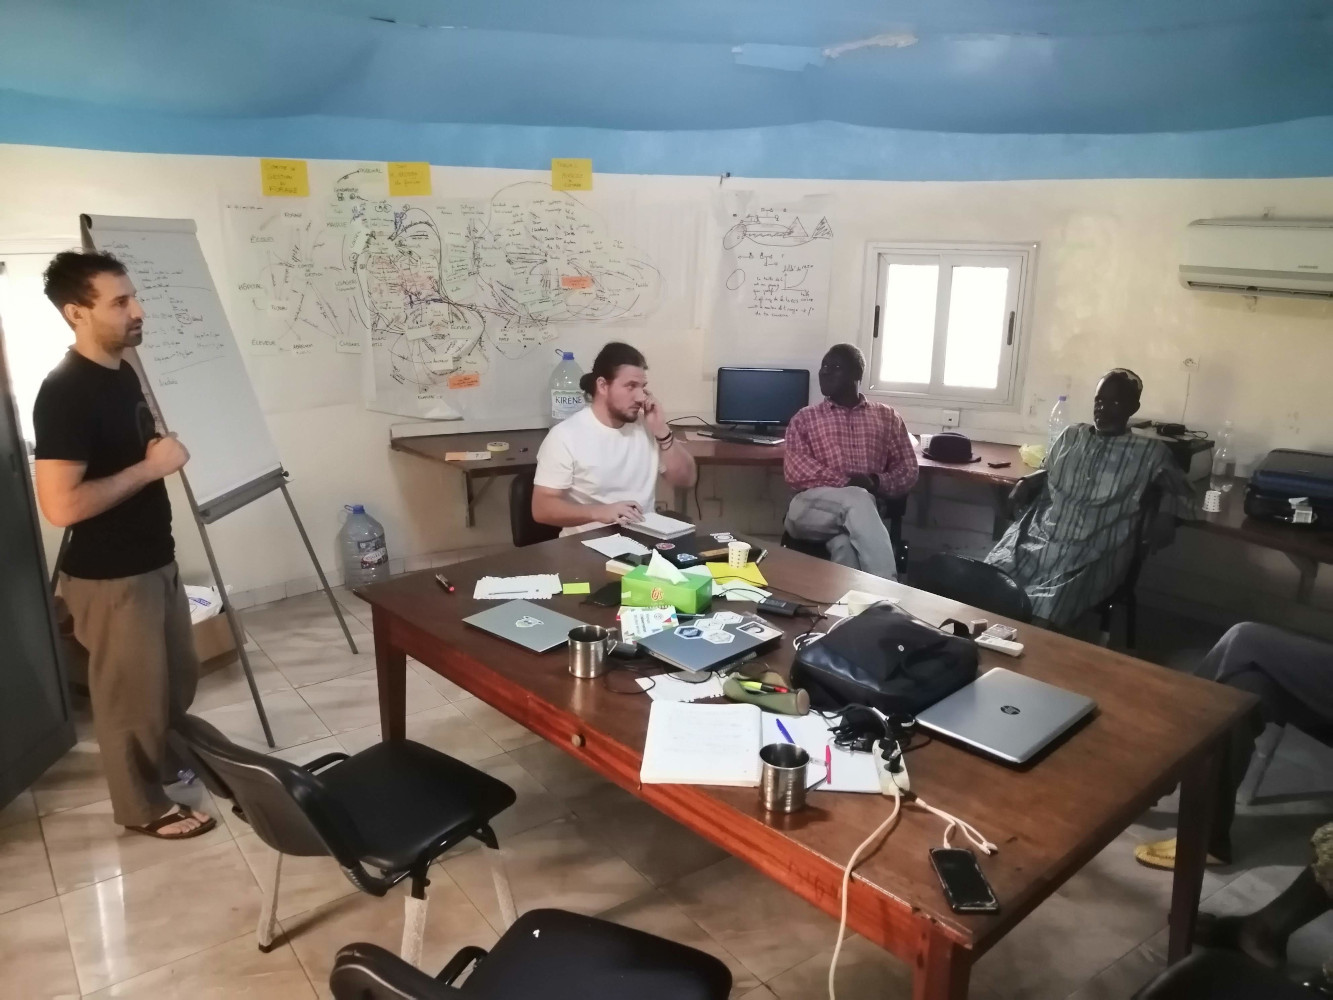
\includegraphics[width=8cm]{img/atelier_niakhar.jpg}
  \end{center}
    %légende de l'image
  \caption{Atelier dans la case de Réunion a Niakar. Sur la photo, sont présent, Romain Reuillon, Paul Chapron, Paul Séné et Marcel Latyr Diouf}
  \label{fig:photoAtelier}
\end{figure}


L'enjeu de cette semaine d'atelier était de formaliser avec les acteurs leur représentation du système d'interaction et de solidarité dans lequel s'inscrit la gestion collective de l'espace à travers la survivance des jachères communautaire. Le système de jachère est lui-même considéré comme un élément clef des processus de maintien de la fertilité des sols et donc un proxy sur les questions de stockage de carbone dans les sols.

À l'issue de la semaine, les participants ont pu valider une première version de leur système qu'on retrouve ici : https://github.com/ElCep/DSCATT/tree/master/PARDi

Ce document à été rédiger avec en s'appuyant sur des notes prise sur le terrain :
\begin{itemize}
  \item Note de Paul : \url{https://hackmd.openmole.org/Rck70wm6Qmu_ztM0M03--w?view}
  \item Note d'Etienne : \url{https://hackmd.openmole.org/qhPAjsJGRbiOQYIItbwPww#}
\end{itemize}


\section{PARDi, un outil de mise en lumière de l'agencement des éléments du système.}

\subsection{Le diagramme comme outil de représentation du système}

La méthode PARDI est une évolution des spécifications de ARDI\cite{etienne_ardi_2011} qui relève de la capacité de l'outil à expliciter des implicites et rendre visible des  hypothèses de modélisation. Cette méthode mobilise des diagrammes pour représenter à la fois les éléments constitutifs du système et les interactions entre ces éléments.

Ces diagrammes sont constitués de noeuds représentés par des cercles ou des ellipses, et d'arcs, représentés par des flèches, qui relient les noeuds.

Dans un diagramme PARDI comme ceux que nous allons inclure dans la suite de ce rapport, les noeuds représentent des acteurs ou des ressources, et les arcs représentent des interactions entre ces acteurs, entre ces ressources ou entre ces acteurs et ces ressources.

%inclusion d'une mage dans le document
\begin{figure}[h!]
  \begin{center}
    
\includegraphics[width=8cm]{img/diagramme_simple.png}
  \end{center}
    %légende de l'image
  \caption{Exemple d'un diagramme simple, ou un acteur A est relié à une ressource B par une interaction.}
  \label{simple_interac}
\end{figure}


Comme les noeuds et les arcs sont nommés, il devient facile de faire une phrase qui décrit l'interaction de façon concise. Par exemple avec la figure \ref{simple_interac} , on pourrait former la phrase suivante : « A consomme B». Plusieurs arcs peuvent exister entre deux mêmes noeuds, pour représenter des interactions différentes.

\section{Modélisation PARDI du système de Diohine}

\subsection{Les Acteurs}

Par la suite nous utiliserons les termes suivants:
\begin{itemize}
  \item \textbf{acteur/role}: personne physique partie prenante dans le système étudié
  \item \textbf{participant} : personnes physiques concourant à la co-construction du modèle durant l'atelier. C'est donc un sous ensemble des "acteurs".
\end{itemize}

\vspace{0.5cm}

La méthode PARDI propose d'interroger des participants évoluant dans un même système. Ils participent à co-construire un diagramme d'interactions entre acteurs sur la base de la connaissance qu'ils ont de ce système. Elle a pour effet de les faire réfléchir sur la réalité du système dans lequel ils évoluent. Les échanges de points de vue stimulent leur créativité en mettant en lumière des liens entre certains objets de leurs quotidiens. L'enjeu du travail de modélisation conceptuel avec PARDI est d'accompagner par un mode de représentation schématique la réflexion sur le fonctionnement du système \cite{becu_les_2010}.\\


Les acteurs représentés dans le modèle sont:
\begin{itemize}
  \item Agriculteur: paysan travaillant la terre et produisant de l'arachide et du mil.
  \item Pasteur: éleveur utilisant les jachères comme pâturage pour son bétail
  \item Chef de cuisine: homme ayant la responsabilité de nourrir tout ou partie de la famille.
  \item Chef de concession (ou chef de famille): homme ayant la charge de la paix sociale au sein de la famille, et donc des différentes cuisines qui la compose.
  \item Notable: personne importante dans le village (ex: instituteur, médecin, imam, etc)
  \item Vieille maman:  femme agée, sage, capable
  \item Chef de village : autorité coutumière du lieu de peuplement, reconnu par l'autorité centrale de l'état.
  \item Conseil municipale : ensemble d'individus qui sont élus aux élections locales et qui s'insèrent dans le droit positif et les institutions de l'état.
  \item Sous-préfet : Représentant de l'état décentralisé sur les territoires. Il prend en charge les conflits quand le droit traditionnel n'a pas réussi à trouver une solution convenable pour les différentes parti du conflit.
  \item Saltigué : voyant et devin qui officie lors de la cérémonie divinatoire de la première chasse. Ses prédictions portent sur la météo, les catastrophes et les remèdes pour y faire face. Un saltigué a un quartier sous sa juridiction
  \item Banque de Céréales : Structure locale (à l'échelle d'un quartier) qui prête des céréales aux agro-pasteurs contre une remboursement ultérieur et vend des céréales. Chaque cuisine contribue au stock de la banque.
\end{itemize}

Les acteurs ci-dessous ne nécessitent pas d'explicitation approfondie, leur nom étant assez explicite.

\begin{itemize}
\item École
\item Revendeur de semence
\item Revendeur d'engrais
\item Animal de trait : âne et cheval
\item Petit ruminant : mouton et chèvre
\item Grand ruminant : boeuf et vache
\end{itemize}

\subsection{L'atelier de modélisation PARDI à Diohine }

Dans le cadre du questionnement autour du stockage de carbone dans les pratiques agricoles du projet DSCATT, nous nous sommes intéréssés à la gestion communautaire de la jachère dans la commune de Diohine.

La jachère est la pratique agricole visant à laisser au repos une parcelle entre deux cultures, généralement sur une période d'un an. À Diohine, cette jachère s'intercale la plupart du temps au sein d'un assolement triénal: Mil, Arachide, Jachère.

Ainsi la jachère a le double avantage de maintenir une fertilité élevée et de stocker du carbone. Ainsi s'intéresser au maintien d'une jachère gérée en commun à l'échelle d est un proxy du stockage de carbone tout en permettant à la population de subvenir à ses besoins alimentaires.

L'atelier de modélisation réunit:
\begin{itemize}
  \item deux agro-pasteurs
  \item un agriculteur
  \item une agri-pastrice vieille maman
\end{itemize}

Ils participent à co-construire le diagramme d'interaction d'un système agro-pastoral à l'échelle de la ville de Diohine, tentant de répondre à la problématique que nous pouvons formuler de la mamnière suivante : «Comment se maintient la jachère communautaire de Diohine ?»

Cette question fait suite à une première consultation à Diohine en mai 2021 lors de laquelle une inquiétude doublée d'une aspiration très forte a été formulée (voir figure \ref{aspiration}) : Comment préserver la jachère communautaire à Diohine ?\cite{perrotton_definition_2021}


\begin{figure}[h!]
  \begin{center}
  %taille de l'image en largeur remplacer "width" par "height" pour régler la hauteur
  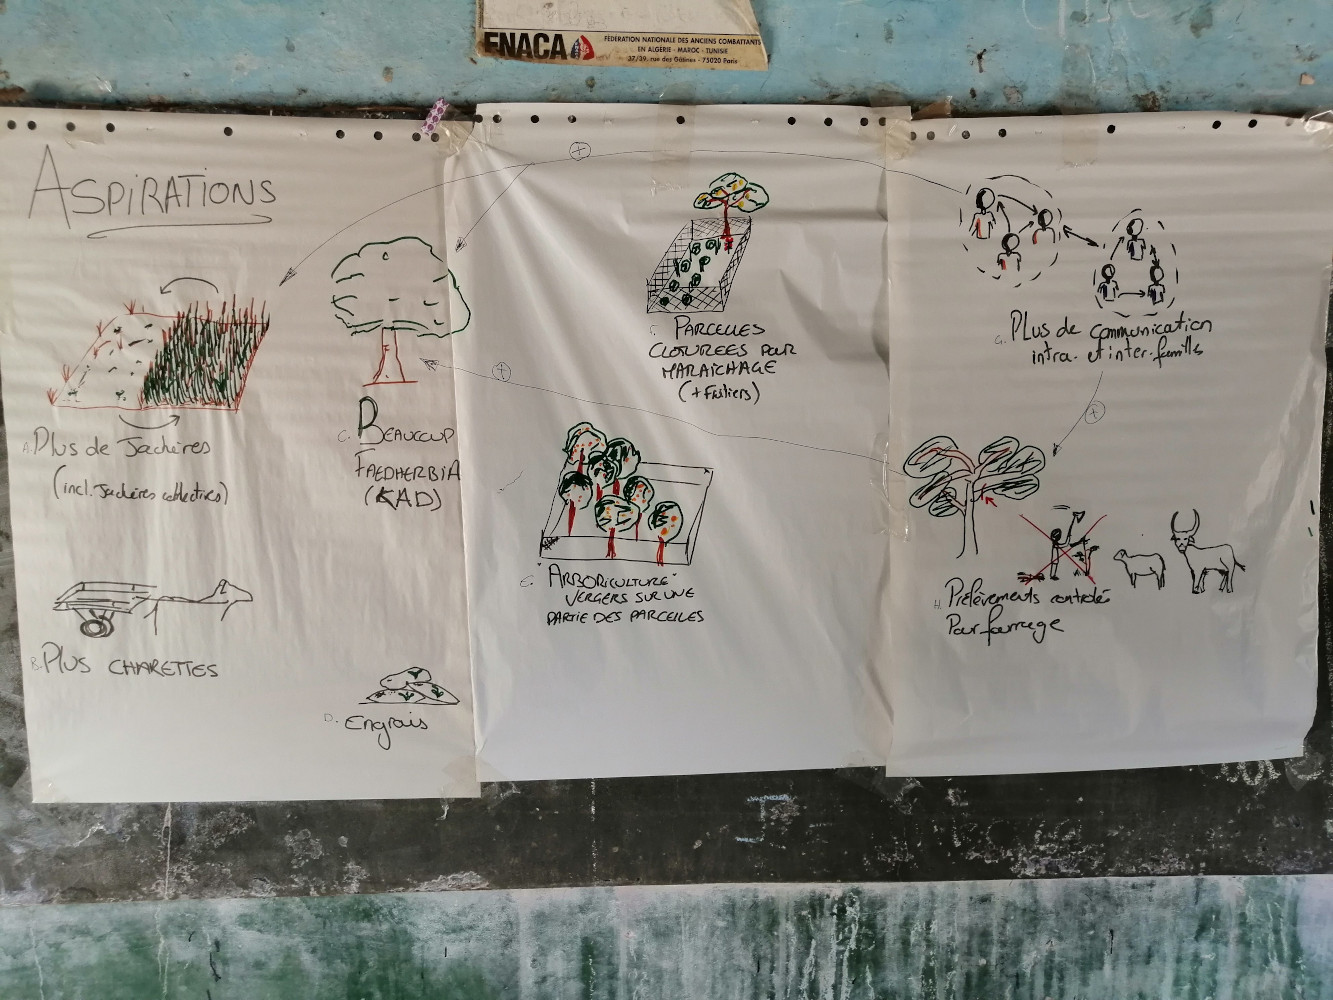
\includegraphics[width=15cm]{img/aspiration_formulee.jpg}
  \end{center}
  %légende de l'image
  \caption{Diagramme des aspirations proposées par un groupe stratégique lors des ateliers d'avril 2021.}
  \label{aspiration}
\end{figure}


Or, pour entrevoir comment préserver cette jachère communautaire à l'avenir, nous devons d'abord nous intéresser à ce qui fonde son existence; et c'est à cette question que nous allons nous intéresser dans les pages suivantes.


Aussi pouvons-nous reformuler cette question en termes plus académiques et généraux de la façon suivante :
Comment préserver une gestion foncière concertée de la fertilité ?



Le travail de modélisation a amené les participants à définir une centaine de nœuds et leurs arcs. Le diagramme complet est visible sur la figure \ref{diagComplet}


\begin{figure}
  \begin{center}
  %taille de l'image en largeur remplacer "width" par "height" pour régler la hauteur
  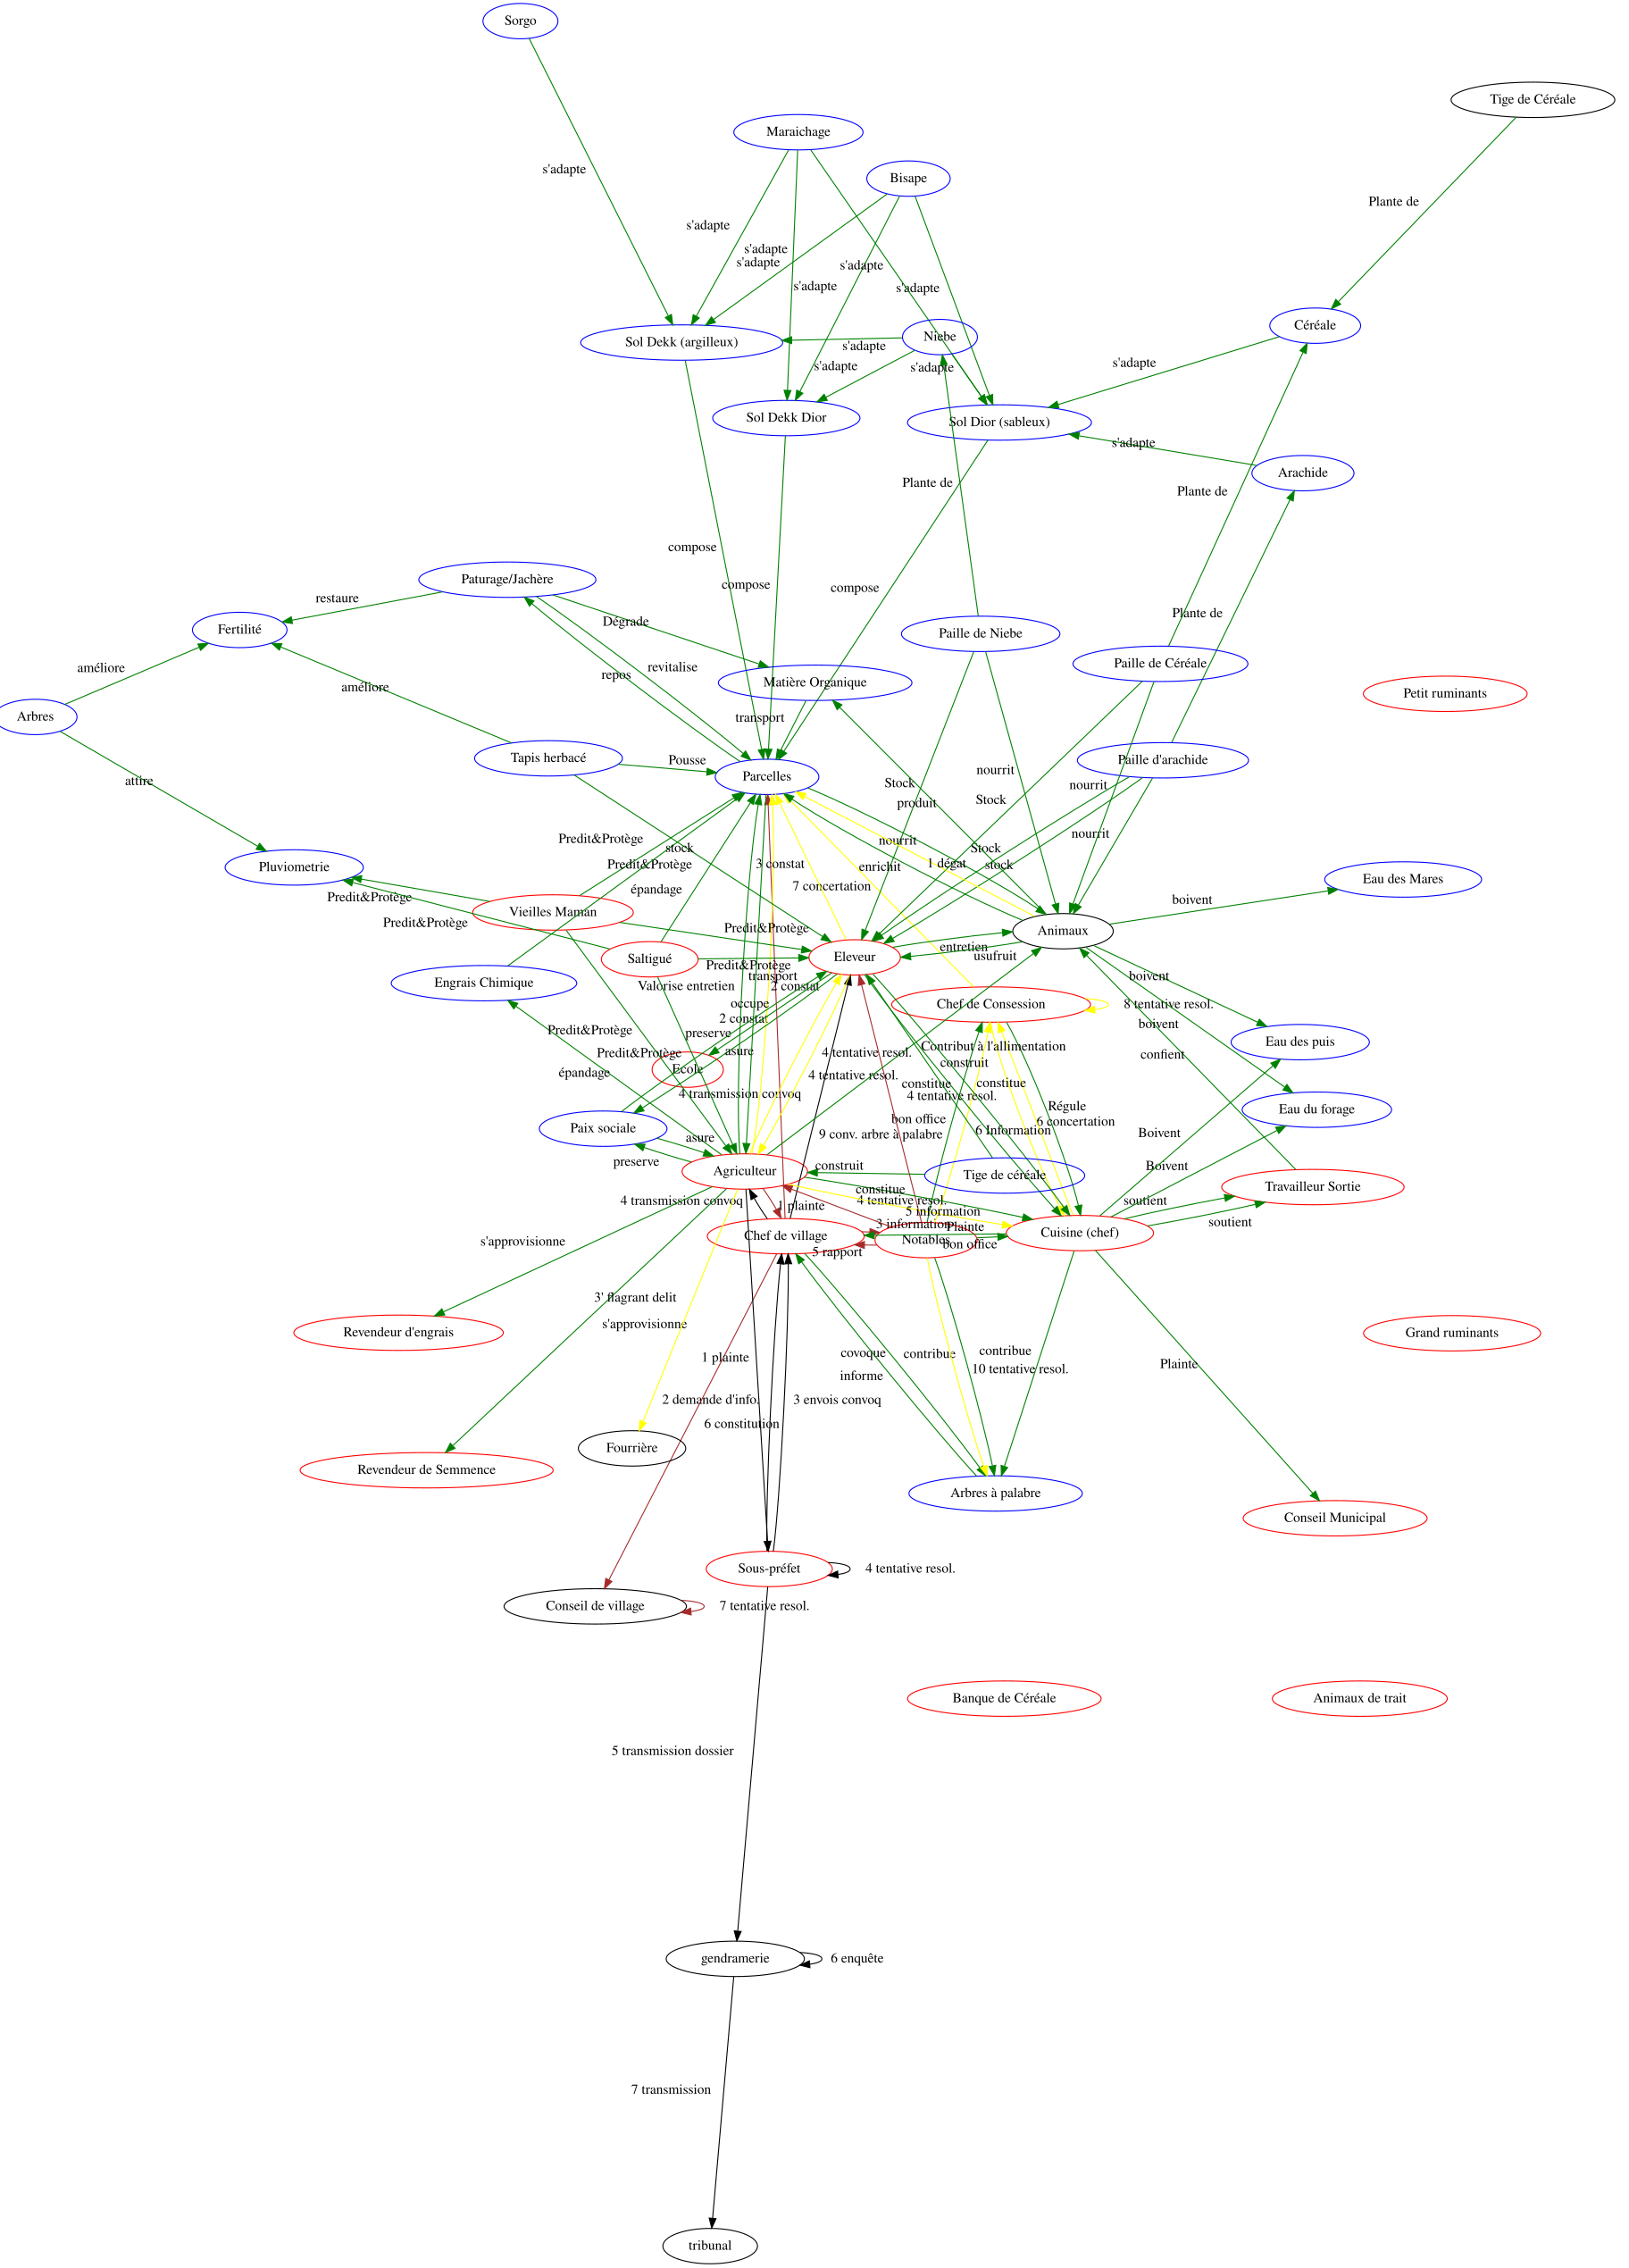
\includegraphics[width=15cm]{img/pardi_fdp.png}
  \end{center}
  %légende de l'image
  \caption{Diagramme complet des interactions relevées pendant l'atelier à Diohine }
  \label{diagComplet}
\end{figure}

Nous avons choisi de le restituer dans ce rapport avec quatre points de vue différents :
\begin{enumerate}
  \item les activités liées au rôle d'agro-pasteur
  \item les mécanismes de résolution de conflit
  \item les interactions liées à la gestion collective de l'espace
  \item les réseaux de solidarités
\end{enumerate}
